\documentclass[a4paper,12pt]{article}

%% Работа с русским языком
\usepackage{cmap}					% поиск в PDF
\usepackage{mathtext} 				% русские буквы в формулах
\usepackage[T2A]{fontenc}			% кодировка
\usepackage[utf8]{inputenc}			% кодировка исходного текста
\usepackage[english,russian]{babel}	% локализация и переносы

%% Отступы между абзацами и в начале абзаца 
\setlength{\parindent}{0pt}
\setlength{\parskip}{\medskipamount}

%% Изменяем размер полей
\usepackage[top=0.5in, bottom=0.75in, left=0.625in, right=0.625in]{geometry}

%% Графика
\usepackage[pdftex]{graphicx}
\graphicspath{{images/}}

%% Различные пакеты для работы с математикой
\usepackage{mathtools}				% Тот же amsmath, только с некоторыми поправками

\usepackage{amssymb}				% Математические символы
\usepackage{amsthm}					% Пакет для написания теорем
\usepackage{amstext}
\usepackage{array}
\usepackage{amsfonts}
\usepackage{icomma}					% "Умная" запятая: $0,2$ --- число, $0, 2$ --- перечисление
\usepackage{bbm}				    % Для красивого (!) \mathbb с  буквами и цифрами
\usepackage{enumitem}               % Для выравнивания itemise (\begin{itemize}[align=left])

% Номера формул
\mathtoolsset{showonlyrefs=true} % Показывать номера только у тех формул, на которые есть \eqref{} в тексте.

% Ссылки
\usepackage[colorlinks=true, urlcolor=blue]{hyperref}

% Шрифты
\usepackage{euscript}	 % Шрифт Евклид
\usepackage{mathrsfs}	 % Красивый матшрифт

% Свои команды\textbf{}
\DeclareMathOperator{\sgn}{\mathop{sgn}}

% Перенос знаков в формулах (по Львовскому)
\newcommand*{\hm}[1]{#1\nobreak\discretionary{}
{\hbox{$\mathsurround=0pt #1$}}{}}

% Графики
\usepackage{tikz}
\usepackage{pgfplots}
%\pgfplotsset{compat=1.12}

% Изменим формат \section и \subsection:
\usepackage{titlesec}
\titleformat{\section}
{\vspace{1cm}\centering\LARGE\bfseries}	% Стиль заголовка
{}										% префикс
{0pt}									% Расстояние между префиксом и заголовком
{} 										% Как отображается префикс
\titleformat{\subsection}				% Аналогично для \subsection
{\Large\bfseries}
{}
{0pt}
{}

% Информация об авторах
\author{Группа лектория ФКН ПМИ 2015-2016 \\
	Анастасия Иовлева \\
	Ксюша Закирова \\
	Руслан Хайдуров}
\title{Лекции по предмету \\
	\textbf{Линейная алгебра и геометрия}}
\date{2016 год}

\newtheorem*{Def}{Определение}
\newtheorem*{Lemma}{Лемма}
\newtheorem*{Suggestion}{Предложение}
\newtheorem*{Examples}{Пример}
\newtheorem*{Comment}{Замечание}
\newtheorem*{Consequence}{Следствие}
\newtheorem*{Theorem}{Теорема}
\newtheorem*{Statement}{Утверждение}
\newtheorem*{Task}{Упражнение}
\newtheorem*{Designation}{Обозначение}
\newtheorem*{Generalization}{Обобщение}
\newtheorem*{Thedream}{Предел мечтаний}
\newtheorem*{Properties}{Свойства}

\renewcommand{\mathbb}{\mathbbm}
\renewcommand{\Re}{\mathrm{Re\:}}
\renewcommand{\Im}{\mathrm{Im\:}}
\newcommand{\Arg}{\mathrm{Arg\:}}
\renewcommand{\arg}{\mathrm{arg\:}}
\newcommand{\Mat}{\mathrm{Mat}}
\newcommand{\id}{\mathrm{id}}
\newcommand{\isom}{\xrightarrow{\sim}} 
\newcommand{\leftisom}{\xleftarrow{\sim}}
\newcommand{\Hom}{\mathrm{Hom}}
\newcommand{\Ker}{\mathrm{Ker}\:}
\newcommand{\rk}{\mathrm{rk}\:}
\newcommand{\diag}{\mathrm{diag}}
\newcommand{\ort}{\mathrm{ort}}
\newcommand{\pr}{\mathrm{pr}}
\newcommand{\vol}{\mathrm{vol\:}}

\renewcommand{\epsilon}{\varepsilon}
\renewcommand{\phi}{\varphi}
\newcommand{\e}{\mathbb{e}}
\renewcommand{\l}{\lambda}
\renewcommand{\C}{\mathbb{C}}
\newcommand{\R}{\mathbb{R}}
\newcommand{\E}{\mathbb{E}}

\newcommand{\vvector}[1]{\begin{pmatrix}{#1}_1 \\\vdots\\{#1}_n\end{pmatrix}}
\renewcommand{\vector}[1]{({#1}_1, \ldots, {#1}_n)}
\begin{document}

\section*{Лекция 10 от 11.02.2016}

\subsection{Расстояние редактирования}

Пусть у нас есть два слова и мы хотим из первого сделать второе. При этом мы можем произвольно расставлять пробелы и заменять буквы. Например:

первое  первое           первое
второе        второе    втор ое
!!!!    !!!!!!!!!!!!    !!! !

Применений полно: проверка орфографии, проверка работ на плагиат (всё несколько сложнее, конечно, но суть примерно такая).

Чуть формализуем: пусть даны строки $s = s_1\ldots s_m$ и $t = t_1\ldots t_n$. Тогда $M$ --- выравнивание --- множество пар $(i,j)$ таких, что $i\in[1,m],\ j\in[1,n]$; также 
$(i_1, j_1)\in M, (i_2, j_2)\in M, i_1 = i_2 \implies j_1 = j_2$

$(i_1, j_1)\in M, (i_2, j_2)\in M, i_1 < i_2 \implies j_1 < j_2$

Расстояние редактирования --- минимальное число операций, переводящее $s$ в $t$. Доступные операции --- удаление букв, добавление букв и замена одной буквы на другую.

Сколько вообще существует возможных выравниваний? Не меньше чем $2^m$ --- каждую из букв первого слова можно изменить, а можно удалить.

Пусть $n=m$; $k$ --- число букв первого слова, сопоставляемых буквам второго слова; тогда $k = |M|$. Получаем, что для фиксировнного $k$ у нас есть $(C_n^k)^2$ выравниваний длины $n$. Всего выравниваний, в таком случае, $\sum\limits_{k=0}^n(C_n^k)^2$.

Или по другому: у нас есть $2n$ букв; из них надо выбрать $k$ из первого слова для замены и $n-k$ из второго для вставки. Тогда всего вариантов $C_{2n}^n$

Пусть $d(s, t)$ --- расстояние редактирования между $s$ и $t$.

$\underbrace{s_1\ldots s_i}\underbrace{\ldots s_m}$

$\underbrace{t_1\ldots t_j}\underbrace{\ldots t_m}$

Рассмотрим первые буквы слов. У нас есть три варианта --- удалить $s_1$ и как-то превратить остаток первого слова во второе; удалить $t_1$ и превратить первое слово в остаток второго; сопоставить $s_1$ и $t_1$ и превратить то, что осталось, друг в друга.

\[
    d(s, t) = \min\begin{cases}
        1+d(s_1\ldots s_m, t) \\
        1+d(s, t_1\ldots t_n) \\
        d(s_1\ldots s_m, t_1\ldots t_n) + (s_1=t_1) \\
    \end{cases}
\]

Базовые случаи: $d(s, <<>>) = |s|; d(`', t) = |t|$

Составим таблицу размером $(m+1)\times (n+1)$.

$\begin{array}{c|ccccccc}
 &6&5&4&3&2&1&0\\
 \text{е}
 \text{о}
 \text{в}
 \text{р}
 \text{е}
 \text{п}
\end{array}$

$T[i][j] = d(s_1\ldots s_m, t_j\ldots t_n)$.

Пользуясь базовыми случаями заполним верхнюю строку и правый столбец. Теперь заполним $T[6][6]$, как минимум из $\{1+T[6][7], 1+T[7][6], T[7][7]+(s_6=t_6)\}$

\begin{lstlisting}
EditDistance(s, t)
    Create T[1..m+1, 1..n+1]
    for k:= 1 to m+1 do
        T[k][n+1] = m+1-k
    for k:= 1 to n+1 do
        T[m+1][k] = n+1-k
    for j:= n downto 1 do
        for i:= m downto 1 do
        T[i][j]:= min{1+T[i+1][j], 1+T[i][j+1], (s[i]!=t[i]) + T[i+1][j+1]}
\end{lstlisting}

А еще можно учитывать траспозиции и получится расстояние Дамерау-Левенштейна:

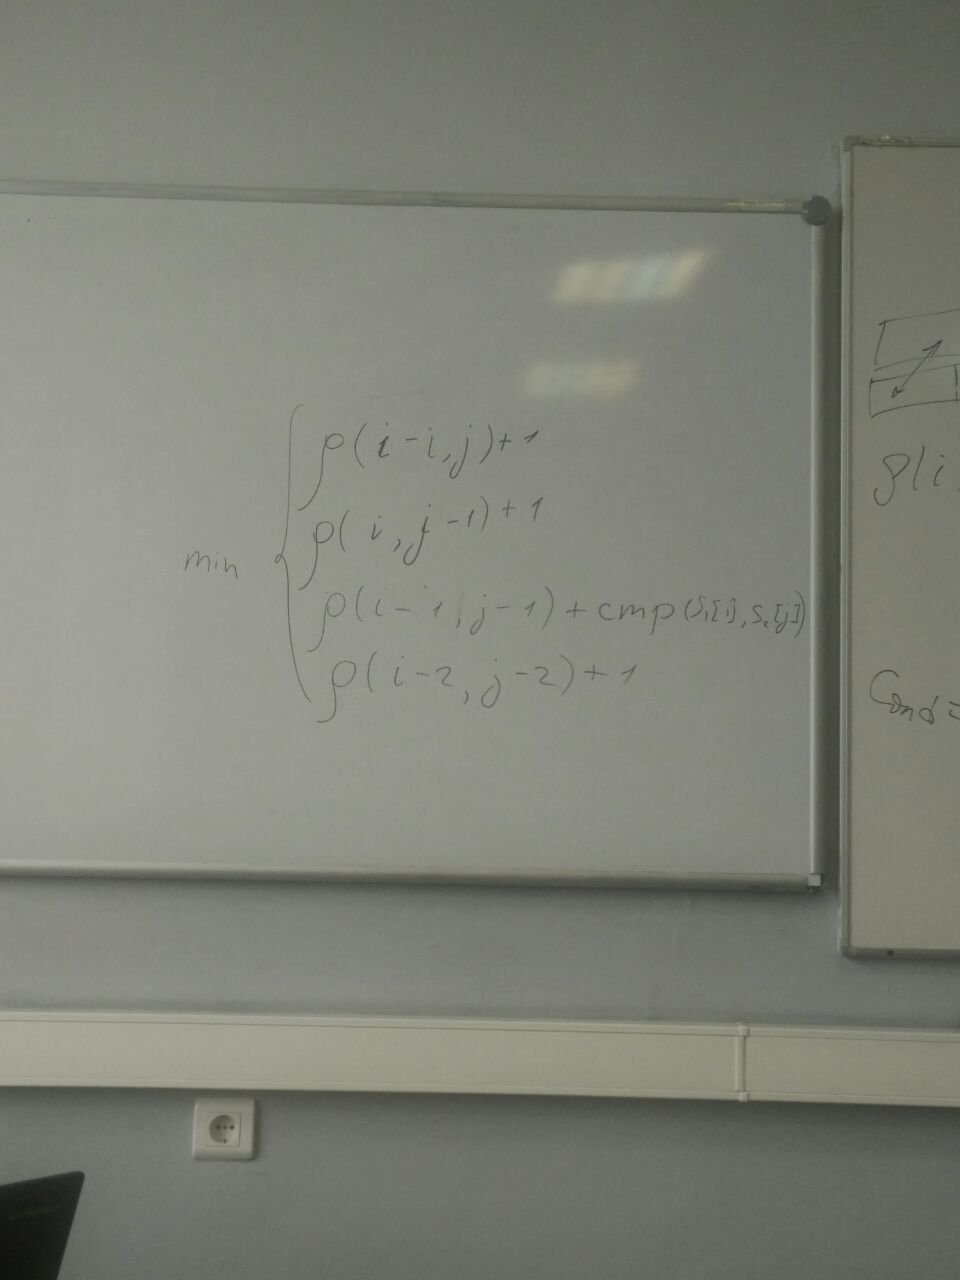
\includegraphics[width=7cm]{10_damerau_1.jpg}
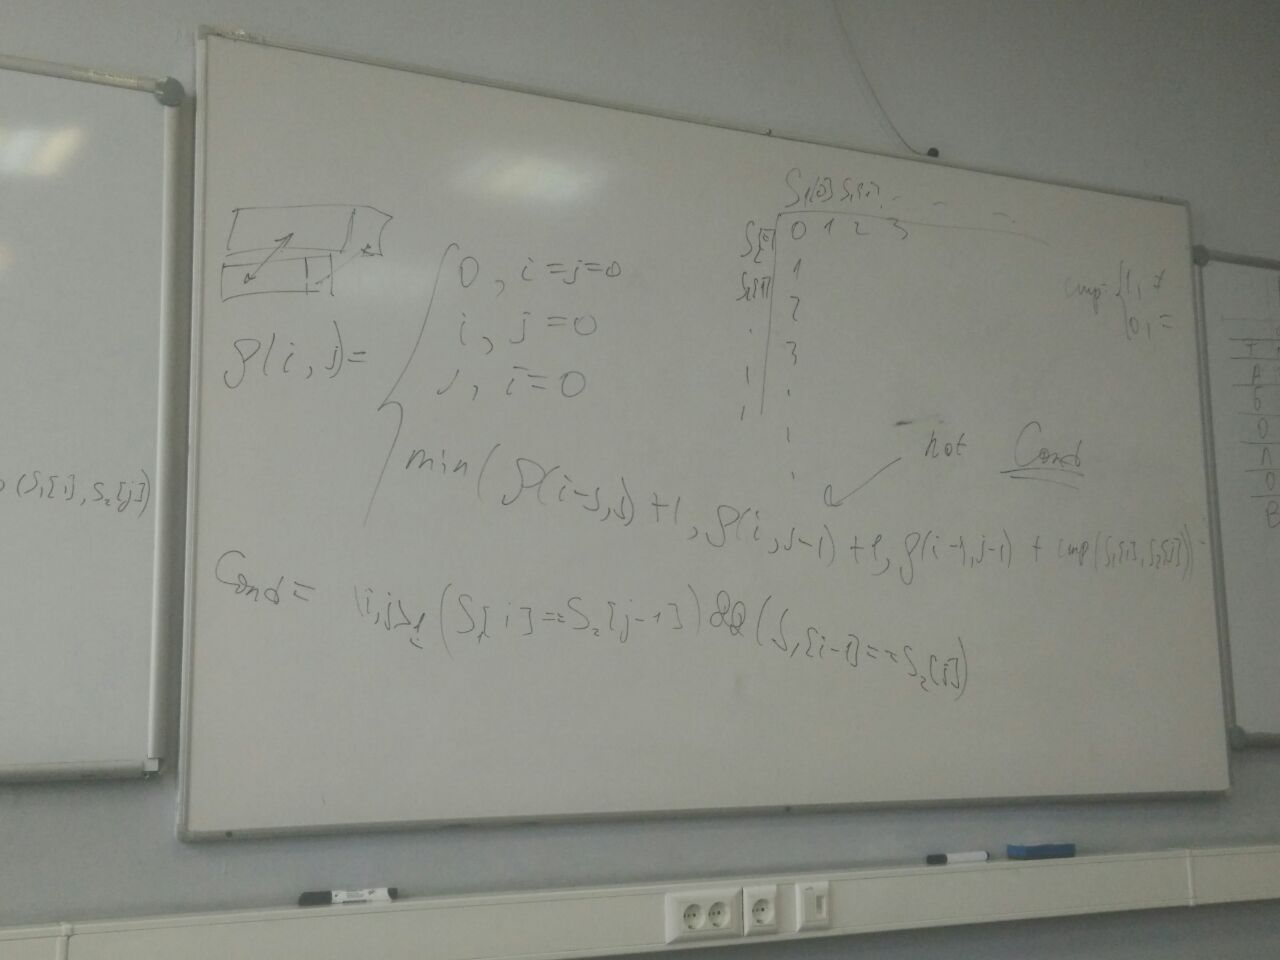
\includegraphics[width=10cm]{10_damerau_2.jpg}

\subsection{Сравнение алгоритмов}

\[
    \begin{array}{c|ccc}
        &\text{Интервалы}&\text{Ширина}&\text{Редактирование}\\
        \text{Число подзадач}&O(n)&O(n)&O(n^2)\\
        \text{Число подзадач, от которых зависит задача}&2&O(n)&3\\
        \text{Время}&O(n)&O(n^2)&O(n^2)\\
    \end{array}
\]

\end{document}
